% !TEX TS-program = xelatex
%
% Created by Chris on 2020-07-19.
% Copyright (c) Chris von Csefalvay, 2020.
\documentclass{article}
\usepackage{amsmath}
\usepackage{polyglossia}
\usepackage{hyperref}

% Bibliography styling
\usepackage[super,square,sort&compress,numbers]{natbib}
\bibliographystyle{unsrtnat}
\usepackage{url}
\urlstyle{same}

% Language and hyphenation
% \usepackage[english]{babel}
\usepackage[htt]{hyphenat}

% Graphics
\usepackage{graphicx}

\hypersetup
{
  pdftitle   = {Statistical dynamics of SARS-CoV-2 as a differential game},
  pdfauthor  = {Chris von Csefalvay}
}

\title{Statistical dynamics of SARS-CoV-2 as a differential game}
\author{Chris von Csefalvay}

\begin{document}

\maketitle

\begin{abstract}
    Abstract
\end{abstract}

\section{Introduction} % (fold)
\label{sec:introduction}
Where an infectious disease is not amenable to population-level prevention through vaccination and risks are non-trivial, non-pharmaceutical interventions (NPIs) remain the principal tool of public health to respond to an outbreak. This is the case with novel infectious diseases that have no specific treatment and no prophylactic (vaccine) available. In the absence of pharmaceutical interventions of proven effectiveness, in particular prophylactically, the main public health response to the emerging pandemic of COVID-19, a viral syndrome caused by the (+)ssRNA virus SARS-CoV-2 (order \emph{Nidovirales}, family \emph{Coronaviridae}, genus \emph{Betacoronavirus}, subgenus \emph{Sarbecovirus}), has rested principally on NPIs, first and foremost social distancing and ancillary steps intended to facilitate that.

In general, any course of conduct that reduces the encounter rate between an individual and other individuals can be considered a form of social distancing. This may be brought about through limiting public facilities for such encounters ('lockdowns'), through limiting individual gatherings by size ('large-gathering bans') and through encouraging individual social distancing. From the perspective of game theory, social distancing can be viewed as a non-cooperative game of a population $P_{1 \ldot n}$ of size $n$, where at any given time $t \in [t_0, t_{e}]$, the strategy adopted by $p_i$ is denoted as $\sigma (p_i, t)$. For the sake of simplicity, we assume that distancing is either not exercised at all or perfectly exercised, i.e. $\sigma (p_i, t) \in \{ 0, 1 \}$. Then, for the entire population, the overall strategy can be described as 

\begin{equation}
	\bar{\sigma}(P, t) = \frac{\displaystyle \sum_{i = 0}^n \sigma(p_i, t)}{n}
	\label{eq:overall_strategy}
\end{equation}

\noindent and for the entire time period, from $t_0$ to the endpoint $t_e$ (which may be eradication, elimination, natural extinction of the pathogen, the availability of a vaccine or a combination thereof), for discrete time $t$,

\begin{equation}
	\bar{\bar{\sigma}}(P) = \frac{\displaystyle \sum_{i = 0}^n \displaystyle \sum_{j = 0}^{t_e - t_0} \sigma(p_i, j)}{n (t_e - t_0)}
	\label{eq:overall_strategy_over_time}
\end{equation}

However, with each course of conduct, there is associated a cost $J(\sigma)$. For simplicity's sake, let us consider these costs to be governed by the following three precepts given a pathogen with fixed characteristics ($R_0$, transmission potential, risks \&c.). Let $\bar{\delta}(P)$ equal the proportion of persons $p \in P$ adopting strategy $\sigma_{\delta}$. It then holds that: 

\begin{enumerate}
	\item A person $p_i \in P$ opting for strategy $\delta$ (social distancing) will incur $c_d$, the immediate costs of distancing. These may be social (lessened social interaction), psychological (lessened access to support systems), economic (lower access to facilities to earn) or simple matters of convenience (access to amenities). While $c_d$ is somewhat dependent on $\bar{\bar{(P)}}$ (thus not distancing does not yield a benefit to a lone social distancer in terms of access to amenities if all of the latter are closed), it can be assumed to be largely constant.
	\item Compared to a person opting for strategy $\delta$, a person $p_i \in P$ opting for strategy $\lnot \delta$ will incur a relative additional risk $f_r(\bar{\delta}(P), t)$, i.e. contingent on the population's behaviour at time $t$.
	\item Finally, a person $p_i \in P$ will regardless of their individual choice (at least at non-trivial population sizes) gain a protective benefit, which is a function of the population's adherence to social distancing. We will denote this term as $f_c(\bar{\delta}(P), t)$.
\end{enumerate}

Then, assigning the variable $c_s$ to represent the cost of illness (economic loss, medical costs, long-term health risks), we can express the cost functions of each strategy, $\sigma_{\delta}$ (social distancing) and $\sigma_{\lnot \delta}$ (no social distancing), as

\begin{equation}
	J_{\sigma_{\delta}}(p_i, t) = c_d - f_c(\bar{\delta}(P), t)
\end{equation}

\noindent and

\begin{equation}
	J_{\sigma_{\lnot \delta}}(p_i, t) = f_r(\bar{\delta}(P), t) c_s - f_c(\bar{\delta}(P), t)
	\label{eq:risk}
\end{equation}

\noindent And consequently, it holds for the population level cost $\bar{J}$ at time $t$ that

\begin{equation}
	\bar{J}(P, t) = \frac{\displaystyle \sum_{i=0}^{\delta(P) n} J_{\sigma_{\delta}}(p_i, t) + \displaystyle \sum_{j=0}^{1-\delta(P) n} J_{\sigma_{\lnot \delta}}(p_j, t)}{n}
	\label{eq:cost_eqn}
\end{equation}

\noindent and for a population over time $t_0$ to $t_e$, 

\begin{equation}
	\bar{\bar{J}}(P) = \int_{t_0}^{t_e} \bar{J}(P, t) dt
\end{equation}

As Reluga (2010) notes, the effect of social distancing diminishes with the increase in participants, the phenomenon of diminishing returns.\cite{reluga2010game} Thus, as the number of individuals in $P$ opting for social distancing increases, the marginal increase by another social distancer diminishes. This can be represented by a discount factor $h$, to yield

\begin{equation}
	\bar{J}(P) = \int_{t_0}^{t_e} e^{-ht} \frac{\delta(P) J_{\sigma_{\delta}}(P, t) + (1 - \delta(P)) J_{\sigma_{\lnot \delta}}(P, t)}{n}
\end{equation}

However, because individual decisions affect the overall gain (due to the component dependent on $\delta(P, t)$), our principal concern is not with individual action but with analysis of such strategies on a population level. This paper will in the following conceptualise infectious disease in a population as a differential game over a differential equation form of the compartmental model first described by Kermack and McKendrick\cite{kermack1927contribution} and, since its publication in 1927, widely adapted and adopted.\cite{vstvepan2007kermack,roberts1999kermack,capasso1978generalization}

% section introduction (end)

\section{Methods} % (fold)
\label{sec:methods}

\subsection{The ordinary differential equations of disease dynamics} % (fold)
\label{sub:the_ordinary_differential_equations_of_disease_dynamics}

Given a population of $n$ under the assumption that reinfection is impossible (as, e.g., in the case of measles) or rare (as is the case for SARS-CoV-2\cite{edridge2020human,deng2020primary,bao2020reinfection}), and neglecting for the time being the vital dynamics (birth, unrelated death, migration) of the population, the dynamics of any population can be modelled as a system of ordinary differential equations

\begin{equation}
	\begin{aligned}
		\frac{dS}{dt} = - \frac{\beta S I}{n} 								\\
		\frac{dI}{dt} = \frac{\beta S I}{n} - \gamma I 						\\
		\frac{dR}{dt} = \gamma I
	\end{aligned}
	\label{eq:sir_equation}
\end{equation}


\begin{figure}
	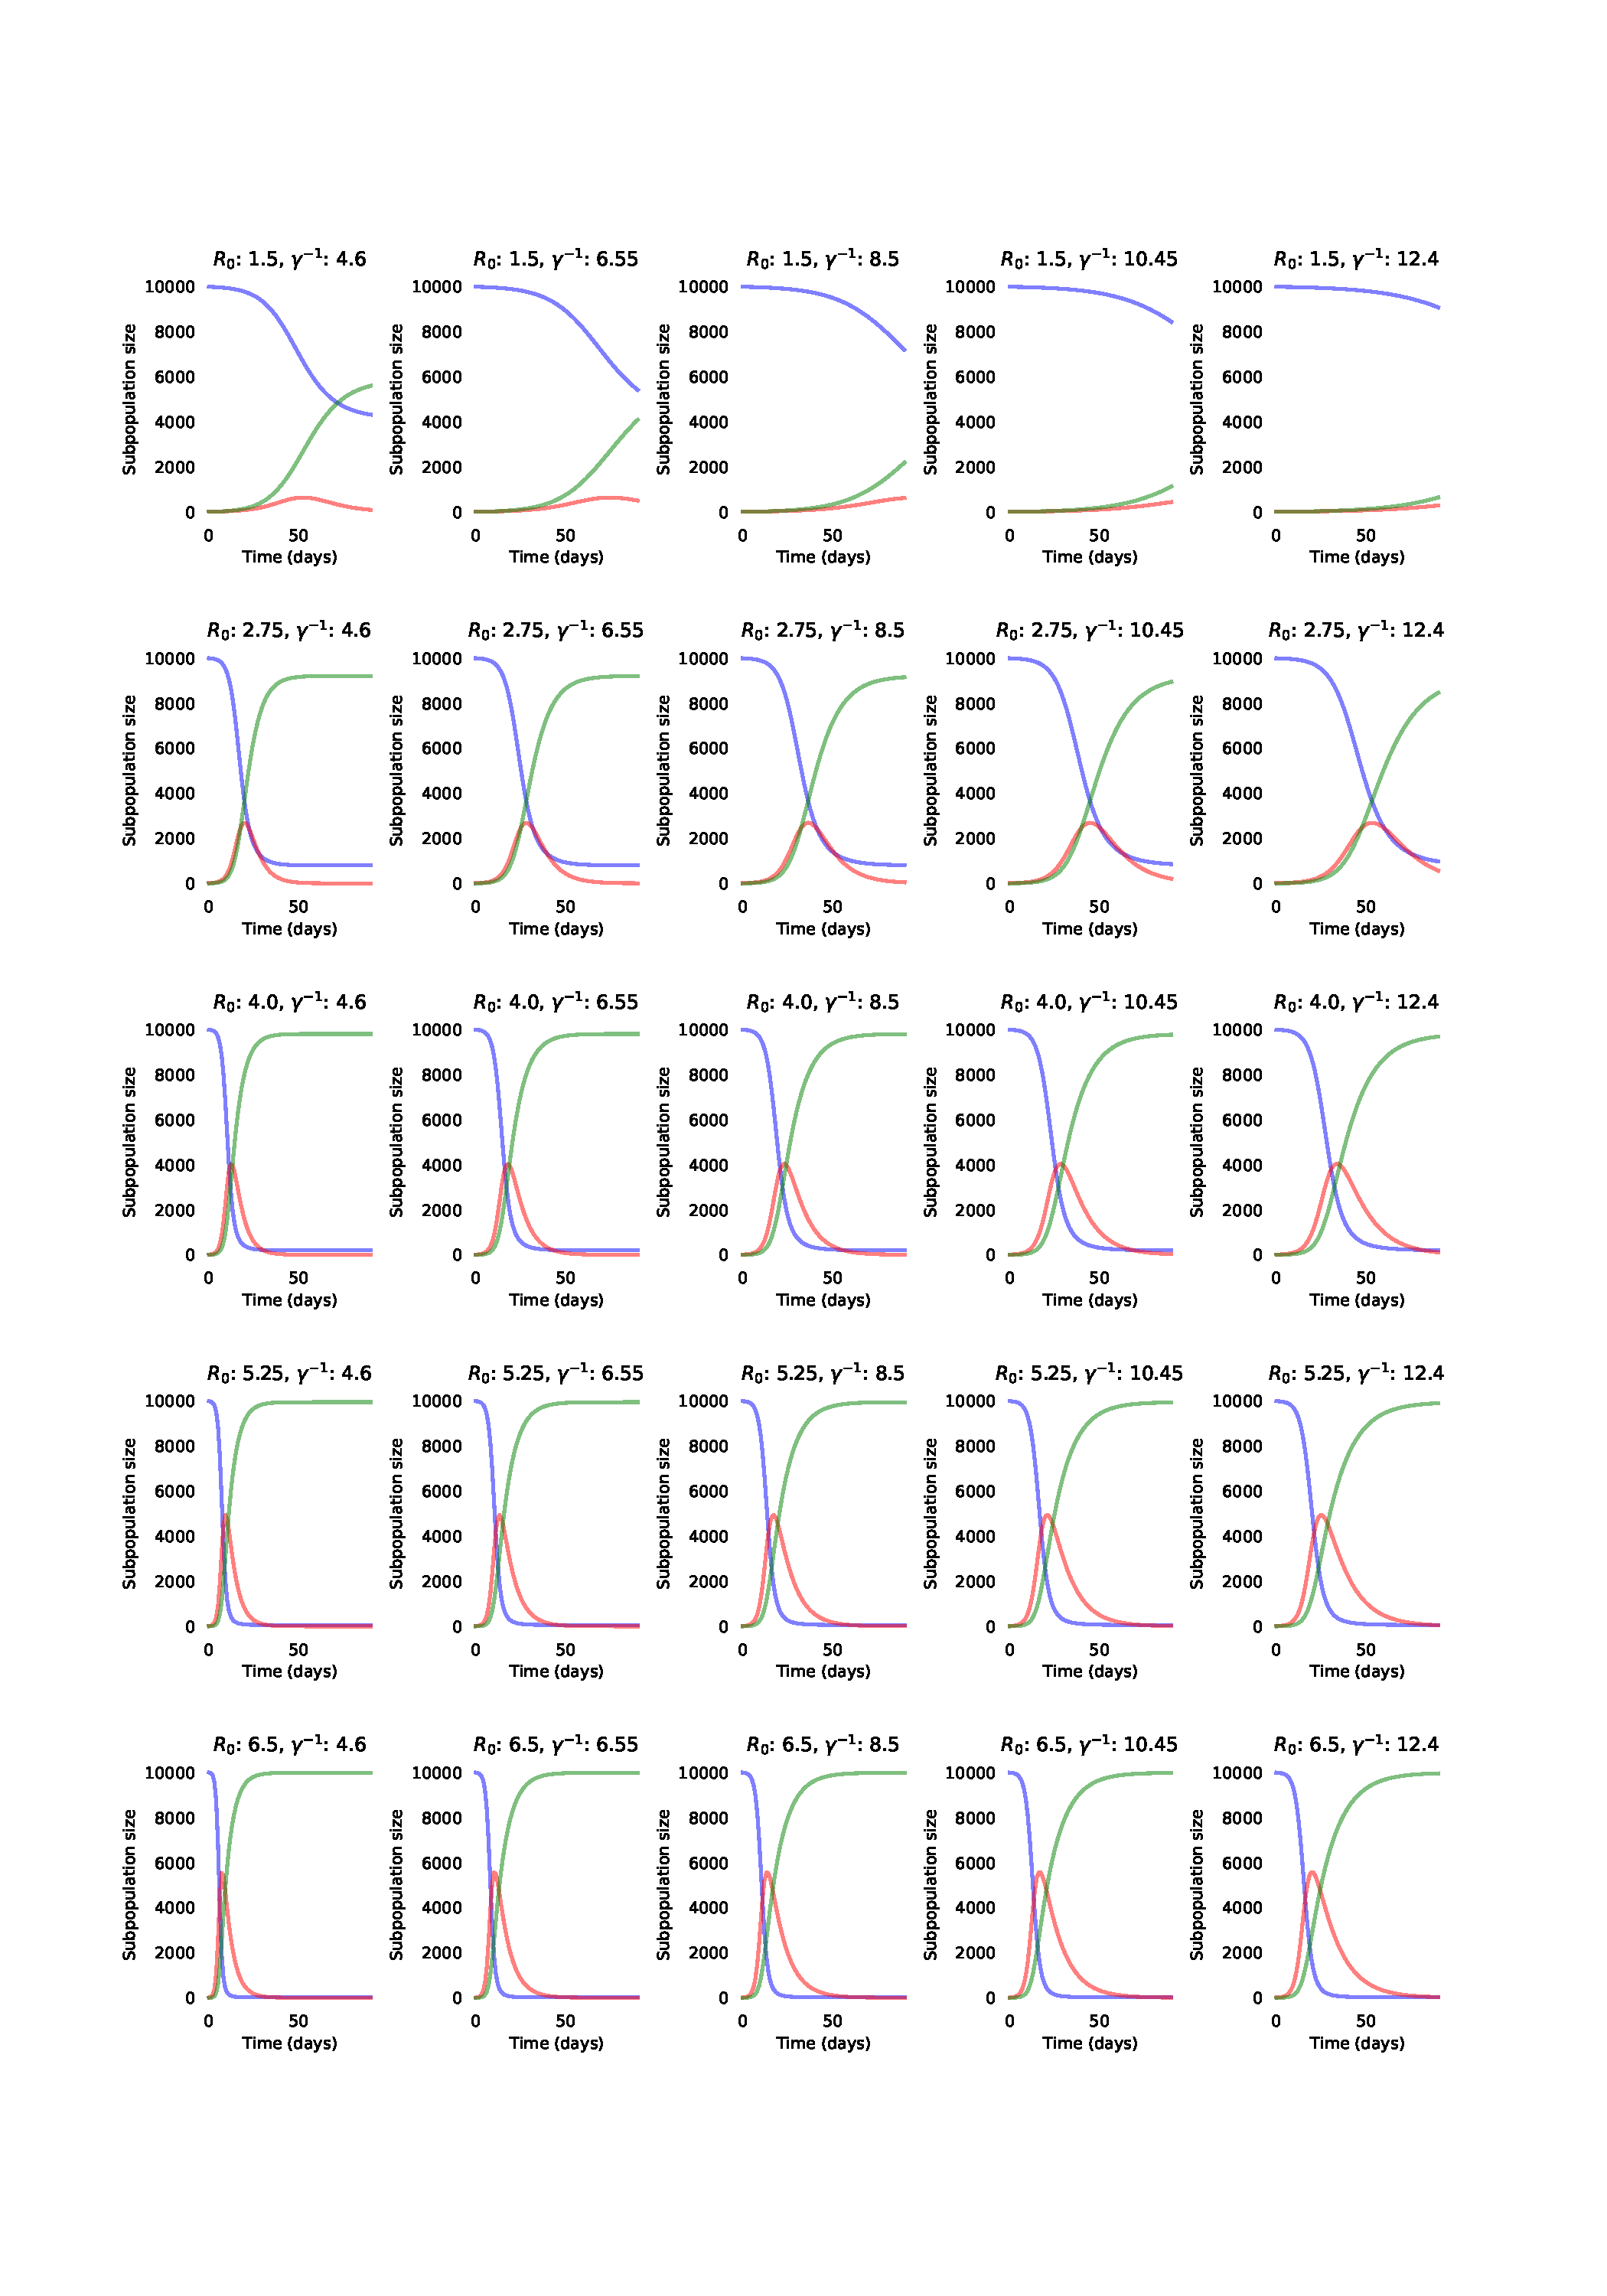
\includegraphics[width=\linewidth]{figures/fig1-odes}
	\caption{Some quantitative solutions for the SIR model's population dynamics over values of $R_0$ between 1.5 and 6.5, and values of $\gamma$ between $1/4.6$ and $1/12.4$ over a base population of 10,000 and a seed population of 0.1\% infected initially. For each plot, $\beta$ is inferred from an $R_0$ value of 2.67, based on Liu et al. (2020),\cite{liu2020reproductive} and the $\gamma$ parameter. The susceptible population is displayed in blue, while infected/infectious cases are marked in red and recovered cases in green.}
	\label{fig:ode_solutions}
\end{figure}

\noindent under the assumption of $S + I + R = 0$, where $S$ represents susceptible individuals, $I$ represents infected/infectious individuals and $R$ accounts for removed individuals (mortality and recovery to immunity). The fraction $\frac{\beta}{\gamma}$ equals the basic reproduction number, $R_0$. For SARS-CoV-2, estimates of $R_0$ range from 1.4 to 6.49, with studies that relied on statistical estimation of $R_0$ ranging from 2.20 to 3.58, with an average of 2.67\cite{liu2020reproductive} $\gamma$, on the other hand, can be estimated as the invers of the number of days of illness, which can be approximated as $8.5 \pm 3.9$ days.\cite{pan2020clinical,liu2020risk} Figure~\ref{fig:ode_solutions} describes some analytical solutions for the differential equations of Equation~\eqref{eq:sir_equation} over a range of plausible values of $R_0$ and $\gamma$ under the assumption of an $R_0$ of 2.67. Even in the absence of firm evidence as to whether SARS-CoV-2 infection followed by recovery would engender lifelong immunity or not,\cite{roy2020covid,ota2020will,lin2020duration} it can be assumed in the short term -- based on evidence from MERS-CoV and SARS-CoV -- that in the short term, survivors remain immune,\cite{prompetchara2020immune} and consequently the number of individuals in $R$ does not decrease. Numerical solutions to this system of differential equations have been calculated using \texttt{odepack} via \texttt{SciPy 1.5.1}\cite{virtanen2020scipy} on Python 3.6, and are presented as Figure~\ref{fig:ode_solutions} for a range of values of $R_0$ and $\gamma$.

% subsection the_ordinary_differential_equations_of_disease_dynamics (end)

\subsection{Population strategy contingent solutions to population dynamics} % (fold)
\label{sub:population_strategy_contingent_solutions_to_population_dynamics}

\begin{figure}
	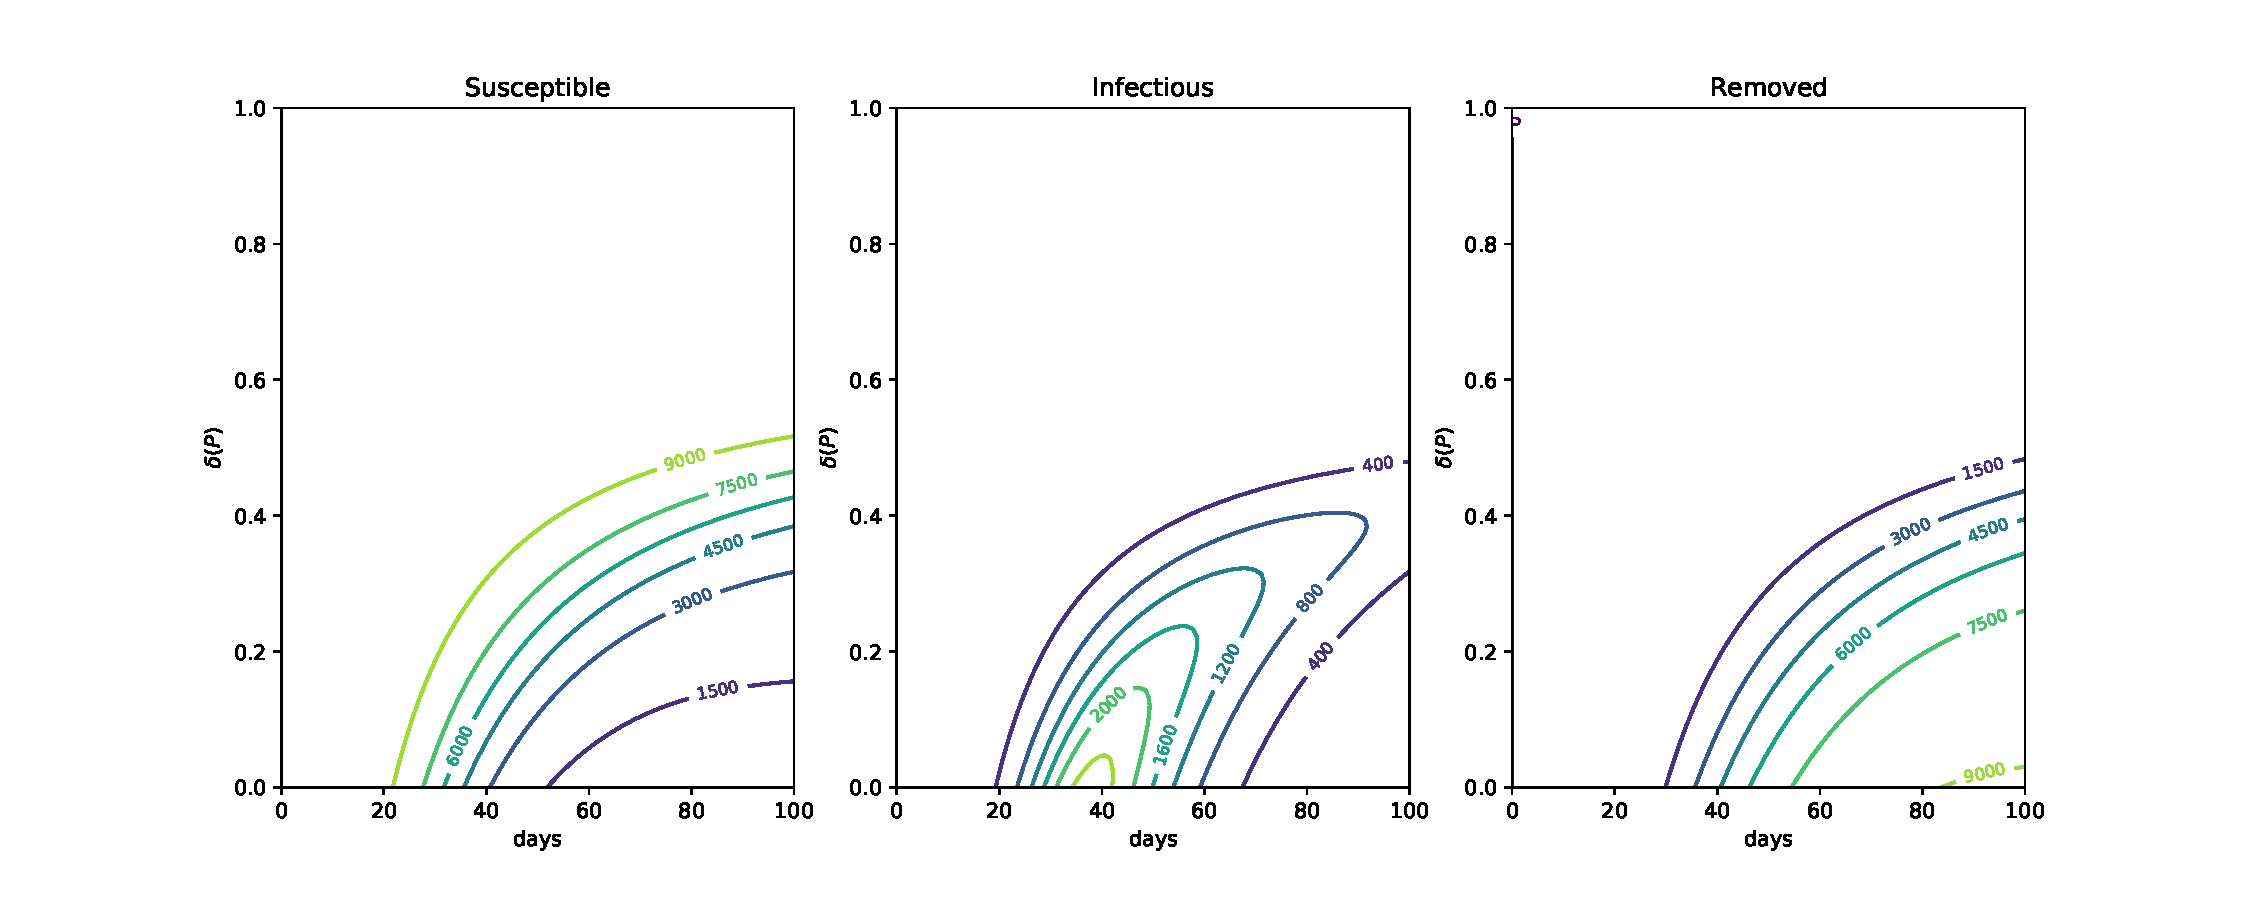
\includegraphics[width=\linewidth]{figures/fig3-SIR-by-delta}
	\caption{Contour diagrams of numeric solutions for susceptible, infectious and removed ($S$, $I$ and $R$) compartment sizes for a base population of 10,000 individuals with a seed population of 0.1\% infected, under the assumption of an $R_0$ of 2.67 and $\gamma$ of $\frac{1}{8.5}$. As this figure indicates, the 'critical mass' of social distancing takes place in the $\delta$ range of 0 to 0.4, and thus even modest increases in social distancing participation at low levels can make a significant difference in the number of infectious cases.}
	\label{fig:fig3-SIR-by-delta}
\end{figure}

Given a population that then adopts a sum strategy $\bar{\sigma}(P, t)$ at time $t$ that results in $\delta(P, t)$ adherence (or in Reluga's terms, investment) to social distancing, the flow from $S$ to $I$ is reduced by a corresponding factor. This allows us to rewrite Equation~\eqref{eq:sir_equation} so that for a society level strategy $\bar{\sigma}$ yielding $\delta$, the populations can be characterised as

\begin{equation}
	\begin{aligned}
		\frac{dS}{dt} = - \frac{\beta S I - \delta \beta S I}{n} 			\\
		\frac{dI}{dt} = \frac{\beta S I - \delta \beta S I}{n} - \gamma I	\\
		\frac{dR}{dt} = \gamma I
	\end{aligned}
	\label{eq:sir_with_social_distancing}
\end{equation}

Solutions to this system of differential equations have been calculated and are presented in Figure~\ref{fig:fig3-SIR-by-delta}. Importantly, this allows us to identify the marginal utility $\hat{U}(P, t)$ as

\begin{equation}
	\begin{aligned}
		\hat{U}(P, t) = \frac{\partial I(P, t)}{\partial \delta(t)}
	\end{aligned}
	\label{eq:marginal_utility}
\end{equation}

\noindent i.e. the partial derivative of $I(P, t)$ over $\delta(P, t)$. Thus, for a population-level strategy $\bar{\sigma}(P, t)$ associated with a compliance rate (i.e. the fraction of persons $p_i \in P$ engaged in social distancing at time $t$) of $\delta(P, t)$, there exists a function $\hat{U}(P, t)$ given $\gamma$ and $R_0$ that indicates the marginal utility at any given value of $\delta(P, t)$. This, too, can be numerically ascertained, and is shown on Figure~\ref{fig:marginal_utility}.

\begin{figure}
	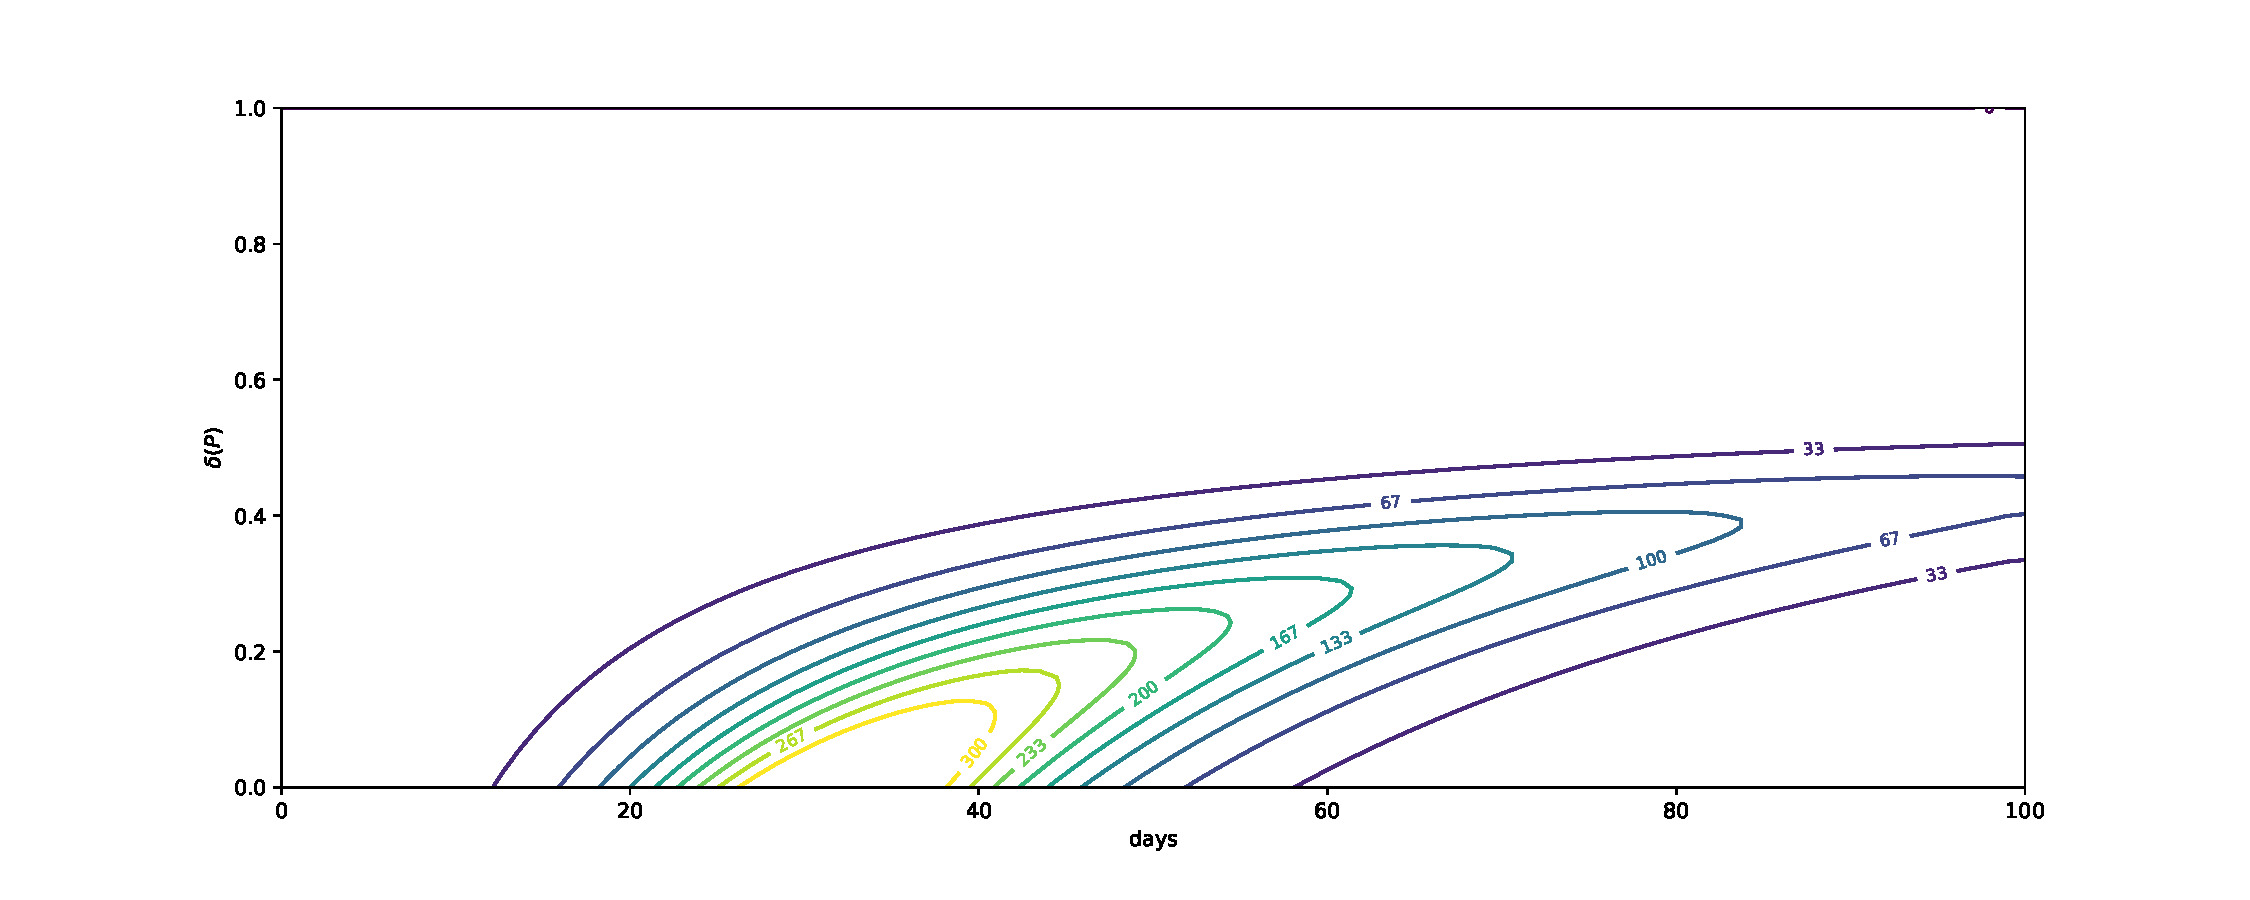
\includegraphics[width=\linewidth]{figures/marginal_utility}
	\caption{Marginal utility of social distancing in a population $P$ of $\delta(P)$ adherence over time. The marginal utility is defined as the vertical component of the gradient of infected individuals. The plot draws on a base population of 10,000 individuals with a seed population of 0.1\% infected, under the assumption of an $R_0$ of 2.67 and $\gamma$ of $\frac{1}{8.5}$.}
	\label{fig:marginal_utility}
\end{figure}

% subsection population_strategy_contingent_solutions_to_population_dynamics (end)

\subsection{Cost, risk and strategy} % (fold)
\label{sub:cost_risk_and_strategy}

Any strategy $\sigma$ has a cost $J(\sigma)$, as stated in Section~\ref{sec:introduction}, and the overall societal cost of $n$ individuals $p_{1 \ldots n} \in P$ each adopting, respectively, strategy $\sigma_{1 \ldots n}$, is $\sum_{i=0}^n J(\sigma_i)$. But since strategies are limited (one may, at any given time, either engage in social distancing or not, assuming for simplicity's sake that those who do so are entirely successful), for any society-level strategy $\bar{\sigma} (t)$ resulting in a level of distancing described by $\delta (t)$, 

\begin{equation}
	\begin{aligned}
		\bar{J}(P, t) = \sum_{i=0}^{\delta(P, t) n} J_{\delta} + \sum_{j=0}^{(1-\delta(P, t)) n} J_{\lnot \delta}
	\end{aligned}
	\label{eq:j_bar}
\end{equation}

\noindent where $J_{\delta}$ is the cost of social distancing for discrete unit time and $J_{\lnot \delta}$ is the cost of not distancing for the same unit time. The latter of these is not constant, as Equation~\eqref{eq:risk} shows, but a function of a constant cost of infection, $c_i$, and the risk of infection ($r_i$), which is contingent on $I(t)$ and $\delta(t)$. Thus, Equation~\eqref{eq:j_bar} can be reformulated (once again, in discrete time) as

\begin{equation}
	\begin{aligned}
		\bar{J}(P, t) = \delta(t) n c_d + (1 - \delta(t)) n J_{\lnot \delta}
	\end{aligned}
\end{equation}

\noindent which expands to

\begin{equation}
	\begin{aligned}
		\bar{J}(P, t) = \delta(t) n c_d + (1 - \delta(t)) n r_i(t) c_i
	\end{aligned}
\end{equation}

For a susceptible individual $p_i \in S$, the risk of infection $r_i(t)$ in discrete time is the proportional likelihood of infection, or in other words, 

\begin{equation}
	\begin{aligned}
		r_i(t) = \frac{\beta S(t) I(t)}{n^2}
	\end{aligned}
\end{equation}

While quantification of costs of illness is difficult, quantification of the economic, social and emotional costs of social distancing is even harder to grasp. However, we may, for a range of cost fractions $\frac{c_d}{c_i}$, estimate values of $\delta(t)$ that denote optimal strategic spaces. Thus, 

\begin{equation}
	\begin{aligned}
		\frac{c_d}{c_i}(P, t) = \frac{(1 - \delta(t)) R_0 \gamma S(t) I(t)}{\delta(t) n^2}
	\end{aligned}
	\label{eq:cost_fraction}
\end{equation}

\begin{figure}
	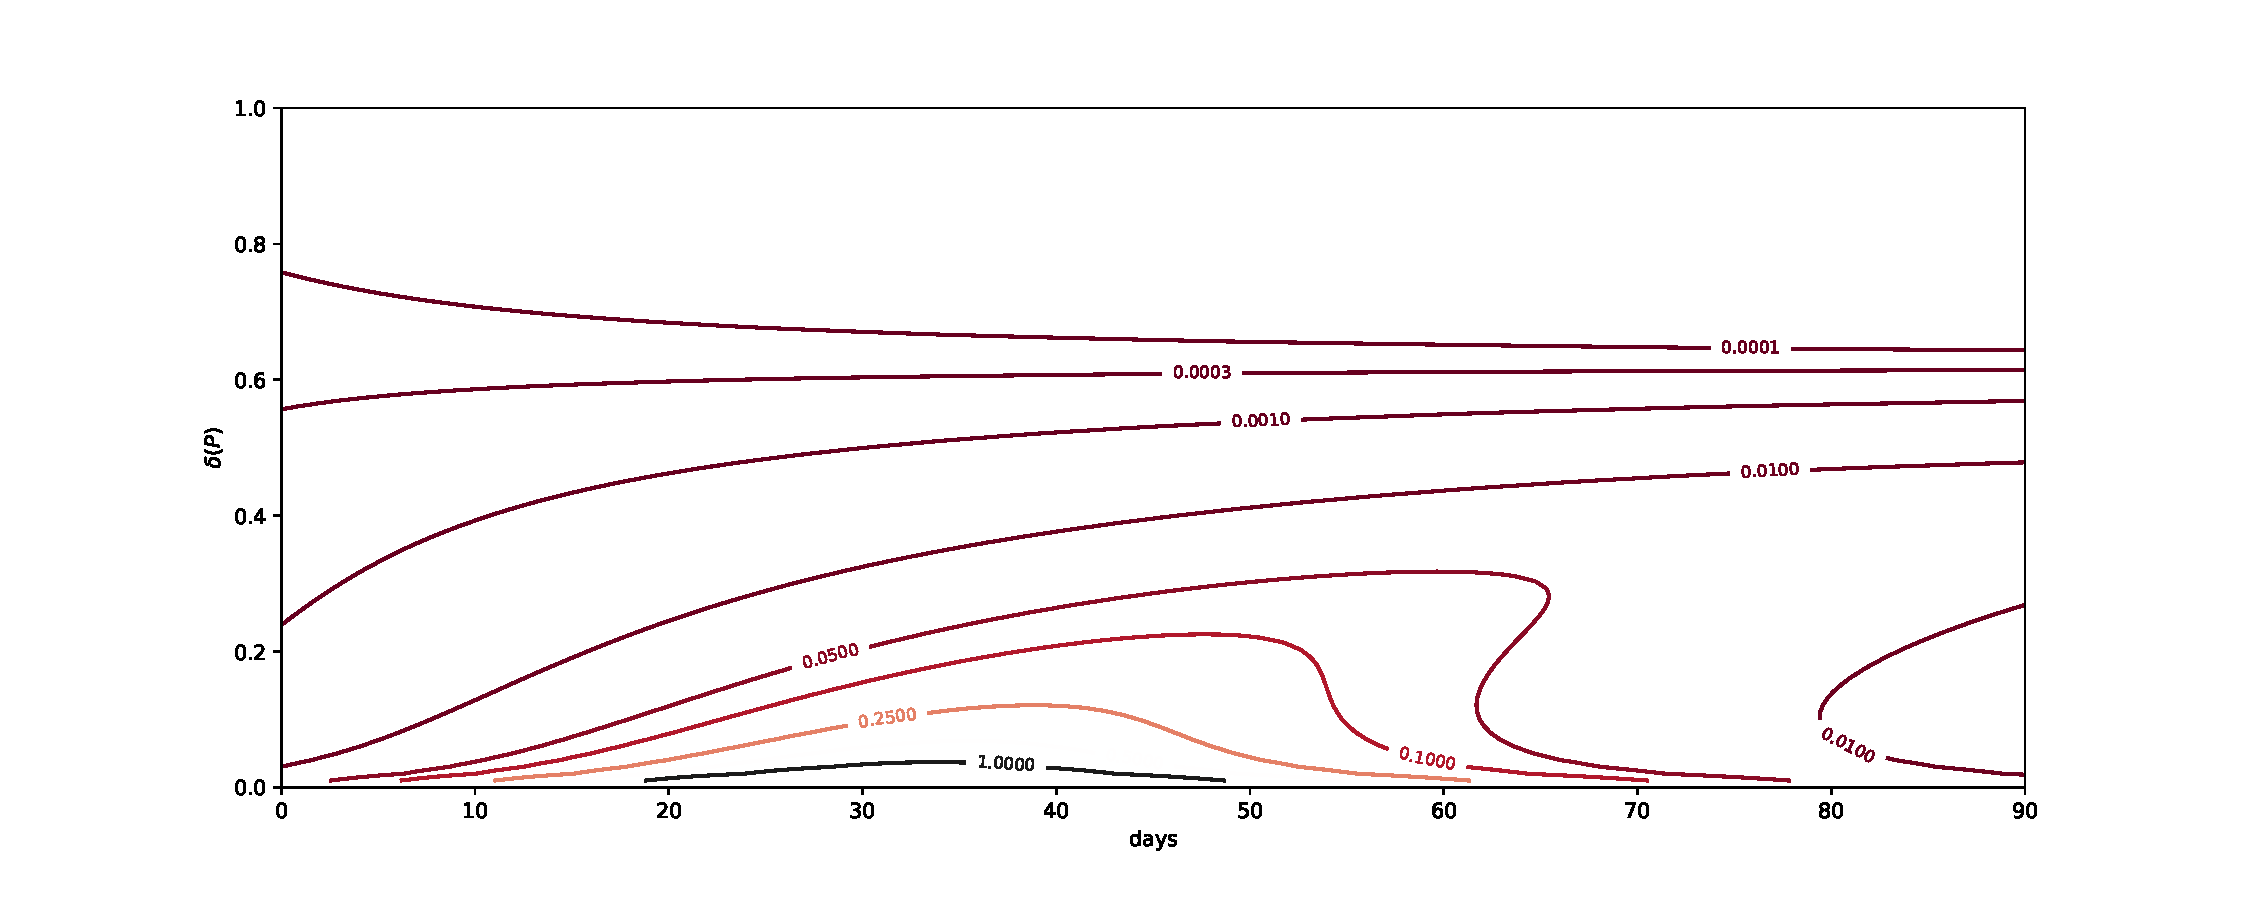
\includegraphics[width=\linewidth]{figures/cost_fraction}
	\caption{Cost fraction $\frac{c_d}{c_i}$ of social distancing in a population $P$ of $\delta(P)$ adherence over time, based on a population of 10,000 individuals with a seed population of 0.1\% infected, under the assumption of an $R_0$ of 2.67 and $\gamma$ of $\frac{1}{8.5}$. The contour lines indicate the cost fraction, i.e. what fraction of the cost of social distancing $c_d$ the cost of illness $c_i$ must be in order to make not distancing a preferred strategy.}
	\label{fig:cost_fraction}
\end{figure}

As numerical estimation of this cost fraction (Figure~\ref{fig:cost_fraction}) shows that for most cases, not distancing can only be a feasible strategy if the cost of distancing very significantly outweighs the cost of illness, often by as much as four orders of magnitude. Since this is notwithstanding risk (i.e. the comparison needs to be made between the absolute cost of infection and the absolute cost of distancing, rather than the probability/risk-adjusted figures).

% subsection cost_risk_and_strategy (end)

% section methods (end)

\section{Results} % (fold)
\label{sec:results}

\subsection{Strategies of social distancing} % (fold)
\label{sub:strategies_of_social_distancing}

As Figure~\ref{fig:fig3-SIR-by-delta} indicates for a given $R_0$ and $\frac{\beta}{\gamma}$, social distancing can have an overwhelmingly significant effect on the number of infectious individuals in a closed population, dependent on the number of persons in the population already engaged in social distancing. This effect is most pronounced early in the epidemic (approx. 2-3 $\gamma^{-1}$ days), and the effect is most significant where less than half of the population is engaged in social distancing. Thus, unlike collective immunity in the case of vaccination, which often necessitates a fairly high level of penetration (typically estimated as $1 - R_0^{-1}$), social distancing can play a meaningful role in particular where much of the population is not engaged in such behaviours. This result can meaningfully inform a policy of encouraging individual social distancing early in an outbreak and dispelling perceptions that unless a critical volume of individuals are participating, marginal action is unnecessary.

% subsection strategies_of_social_distancing (end)

\subsection{Marginal utility of social distancing} % (fold)
\label{sub:marginal_utility_of_social_distancing}

Based on the key epidemiological dynamics data on the SARS-CoV-2 pandemic, the highest marginal effect of social distancing takes place in the same early timeframe of approx. 2-3 $\gamma^{-1}$ days. Unsurprisingly, even without integrating the time-dependent discount factor proposed by Reluga (2010), the numerical solutions indicate that the effect of social distancing is most significant where it is not yet a widely adopted strategy: for SARS-CoV-2, based on an initial population of 10,000 with a seed population of 0.1\% infected, the greatest marginal utility is encountered where less than 20\% of the population is engaged in such behaviour, and the effect is significantly less noticeable once $\delta(P)$ reaches 0.5.

Calculations of marginal utility matter because they can guide public policy in determining what fraction of the population may feasibly be exempted from social distancing. Given the need for critical services to continue even in the throes of a pandemic, marginal utility calculations based on empirical data on an outbreak itself, as well as the societal response (as expressed by $\delta(P, t)$), may contribute to more accurate public health measures while limiting the effect of such measures on the economy. 

% subsection marginal_utility_of_social_distancing (end)

\subsection{Costs and strategy choices} % (fold)
\label{sub:costs_and_strategy_choices}

The costs both of social distancing and of failing to do so are notoriously difficult to quantify accurately. Indeed, many of these costs are by their very nature not amenable to quantification. At the same time, by quantifying the relative ratio of cost of distancing ($c_d$) and cost of illness ($c_i$), we can identify a strategy-associated cost relationship that, given solid information, can assist in societal decision-making as to social distancing. As Figure~\ref{fig:cost_fraction} shows, for most cases, the cost of social distancing would have to exceed the cost of illness by at least an order of magnitude to make it a preferable strategy. In addition, the computational solution of Equation~\eqref{eq:cost_fraction} shows not only that failure to socially distance may only be a preferable choice if the costs of distancing vastly exceed the costs of illness, but that this remains the case for much of the short term (<90 days). 

% subsection costs_and_strategy_choices (end)

% section results (end)

\section{Discussion} % (fold)
\label{sec:discussion}

Pandemics pose a significant challenge to public health and social decision-making, and the COVID-19 pandemic is by no means an exception. Non-pharmaceutical interventions, such as social distancing, play a significant role in the public health arsenal and may play a determinative role in stemming the tide of an infectious disease that is otherwise not amenable to treatment or prophylaxis. Thus, until a vaccine or a reliable therapeutic, ideally with prophylactic properties, is found, non-pharmaceutical interventions are the mainstay of public health activity in the face of COVID-19.

This paper discussed a subject that is not devoid of controversy, both in the scientific and in the public realm. By their nature, non-pharmaceutical interventions interfere with citizens' day-to-day lives and may have complex economic, social and psychological effects. It is therefore important that strategy options are adequately explored from a quantitative perspective. It is hoped that in reinforcing the case for social distancing through an analysis of the statistical dynamics that underlie it, this paper can add to the wealth of literature in support of social distancing as an effective and cost-efficient non-pharmaceutical intervention where other tools are unavailable or inappropriate.

% section discussion (end)

\section*{Competing interests} % (fold)
\label{sec:competing_interests}

The author declares no competing interests.

% section competing_interests (end)

\section*{Supplementary data} % (fold)
\label{sec:supplementary_data}

All simulations, code and data are available on Github and under the DOI XXXXXXX.

% section supplementary_data (end)

\bibliography{bibliography}

\end{document}
